%Primera Unidad
\section{Preliminares del cálculo}
\begin{frame}[allowframebreaks]{Teoremas Preliminares}
Esta presentación esta basada en el texto de \textcolor{gray}{\cite{burden2017análisis}}.
\label{RetornoTeoremaPreliminares1}
\begin{block}{Criterio del límite}
Sea $f:\mathbb{R}:\rightarrow \mathbb{R}$. Asuma que $\lim_{x\rightarrow \infty}f(x)$ existe y es igual a $L$. Entonces la sucesión $\{a_n\}=\{f(n)\}$ converge a $L$ también.  
\end{block}
\hyperlink{CriterioLimite}{\textcolor{cyan}{Enlace a ejercicio.}}
\begin{block}{Teorema de convergencia monótona}
Suponga que la sucesión $\{a_n\}$ es monótona creciente y acotada superiormente, entonces $\{a_n\}$ es convergente.
\end{block}
\hyperlink{ConvergenciaMonotona}{\textcolor{cyan}{Enlace a ejercicio.}}
\begin{block}{Teorema del sándwich}
Suponga que $\{a_n\}$ y $\{b_n\}$ convergen al valor de $L$. Además asuma que
$$a_n\leq x_n\leq b_n,$$
para $n>N$ para algún $N$ fijo; entonces $\{x_n\}$ converge a $L$.
\end{block}
\hyperlink{Sandwich}{\textcolor{cyan}{Enlace a ejercicio.}}
\framebreak
\label{RetornoTeoremaPreliminares2}
\begin{block}{Teorema del valor medio}
Si $f\in C[a,b]$ y $f$ es diferenciable en $(a,b),$ entonces existe un número $c$ en $(a,b)$ con
$$f'(c)=\dfrac{f(b)-f(a)}{b-a}.$$
\end{block}
\begin{figure}[H]
\begin{center}
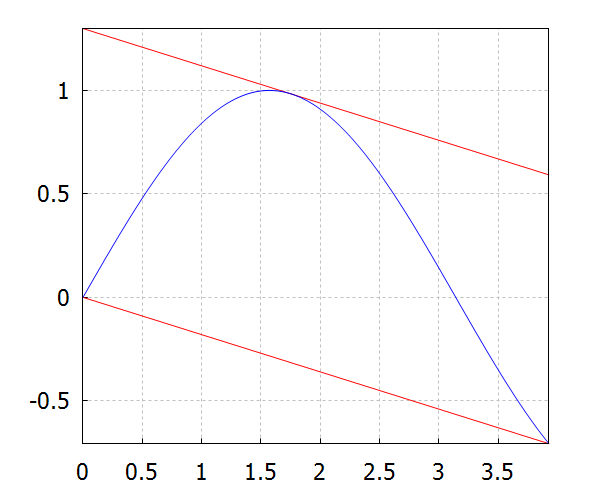
\includegraphics[scale=0.5]{Imagen17}
\end{center}
\caption{En la figura se puede ver un ejemplo con $f(x)=\sin(x)$ para $x\in \bigg[0,\dfrac{5\pi}{4}\bigg]$}
\end{figure}
\framebreak
\vspace*{-0.7cm}
\label{RetornoTeoremaPreliminares3}
\begin{block}{Teorema del valo extremo}
\begin{itemize}
\item Si $f\in C[a,b]$, entonces existe $c_1,c_2\in [a,b]$ con
$$f(c_1)\leq f(x)\leq f(c_2)$$
para $x\in[a,b]$.
\item Si además $f$ es diferenciable en $(a,b)$, entonces $c_1$ y $c_2$ son iguales a los extremos ($a$ o $b$) o los lugares donde la derivada se hace cero en $(a,b)$. 
\end{itemize}
\hyperlink{EjercicioExtremos}{\textcolor{cyan}{Enlace a ejercicio}}
\end{block}
\begin{figure}[H]
\begin{center}
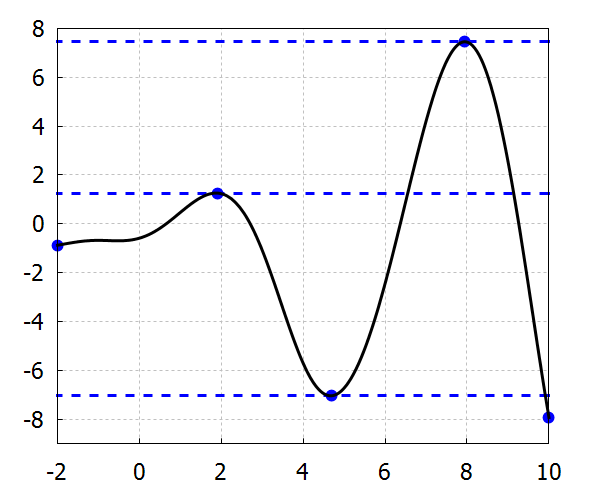
\includegraphics[scale=0.4]{Imagen18}
\end{center}
\caption{Se puede apreciar en el ejemplo, que el máximo de la función se alcanza en un lugar donde la derivada es cero y el mínimo en el extremo derecho.}
\end{figure}
\framebreak
\label{RetornoTeoremaPreliminares4}
\begin{block}{Teorema del valor intermedio}
Si $f\in C[a,b]$ y $K$ es cualquier número entre $f(a)$ y $f(b)$, entonces existe un número $c$ en $(a,b)$ para el cual $f(c)=K$.
\end{block}
\hyperlink{EjercicioIntermedio}{\textcolor{cyan}{Enlace a ejercicio}}
\begin{figure}[H]
\begin{center}
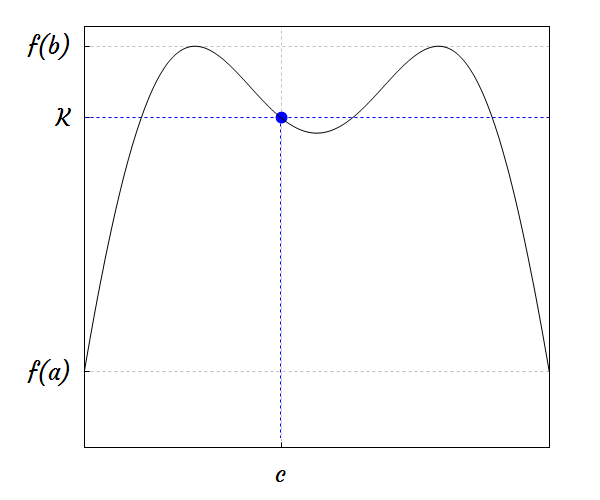
\includegraphics[scale=0.7]{Imagen19}
\end{center}
\end{figure}
\framebreak
Se define $C^n[a,b]=\{f:[a,b]\rightarrow \mathbb{R}| f,f',\cdots,f^{(n)}\text{ son continuas en }[a,b]\}.$
\label{RetornoTeoremaPreliminares5}
\begin{block}{Teorema de Taylor}
Supong que:
\begin{itemize}
\item $f\in C^n[a,b]$.
\item $f^{(n+1)}$ esta definida en $[a,b]$.
\item $x_0\in[a,b]$.
\end{itemize} 
Entonces, para cada $x\in[a,b]$, existe $\xi(x)\in (x_0,x)$ (si $x>x_0$ y $\xi(x)\in(x,x_0)$ en el otro caso)  tal que: 
\begin{itemize}
\item $f(x)=P_n(x)+R_n(x)$ donde
\item $P_n(x)=\displaystyle \sum_{k=0}^{n}\dfrac{f^{(k)}(x_0)}{k!}(x-x_0)^k$ y
\item $R_n(x)=\dfrac{f^{(n+1)}(\xi(x))}{(n+1)!}(x-x_0)^{(n+1)}$.
\end{itemize}
\end{block}
\hyperlink{EjercicioTaylor}{\textcolor{cyan}{Enlace a ejercicio}}
\end{frame}
\section{Raíces de ecuaciones}
\begin{frame}[allowframebreaks,fragile]{Raíces de ecuaciones}
\label{RetornoTeoremaRaices1}
\begin{figure}[H]
\begin{center}
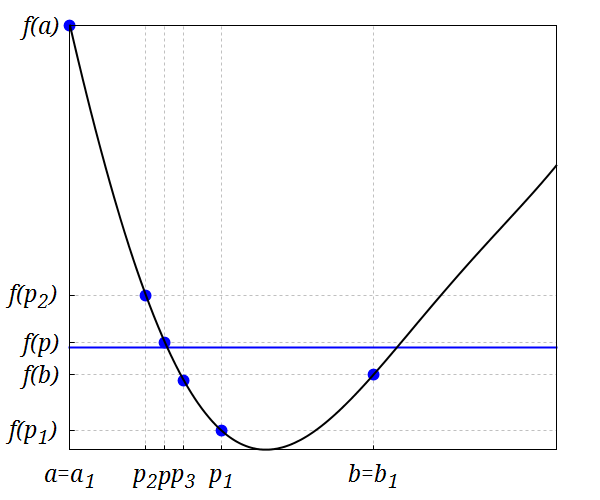
\includegraphics[scale=0.7]{Imagen20}
\end{center}
\caption{\textbf{Método de Bisección: }En la figura se muestra el mécanismo de la bisección.}
\end{figure}
\label{RetornoTeoremaRaices2}
\begin{lstlisting}[caption=''Método de Bisección'',style=mystyle,language=octave,numbers=left]
function x=Biseccion(f,a,b,TOL,N0)
  i=1;FA=f(a);
  while(i<=N0)
    p=a+(b-a)/2;
    FP=f(p);
    if(FP==0 || (b-a)/2<TOL)
      x=p;
      break;
    endif
    i=i+1;
    if(FA*FP>0) 
      a=p;
      FA=FP;
    else
      b=p;  
    endif
  endwhile
  if(i>N0)
    x=inf;
  endif
endfunction
\end{lstlisting}
\label{RetornoTeoremaRaices3}
\begin{block}{Teorema de convergencia del método de bisección}
Supongamos que $f\in C[a,b]$ y $f(a)f(b)<0$. El método de bisección genera una sucesión $\{p_n\}$ que aproxima a un cero de $p$ de $f$, tal que:
$$|p_n-p|\leq \dfrac{b-a}{2^n}.$$
\hyperlink{EjercicioBiseccion}{\textcolor{cyan}{Enlace a ejercicio}}
\end{block}
\textcolor{red}{
\indent Primero note que $p\in [a_n,b_n]$ (teorema del valor intermedio), entonces $$|p-(a_n+b_n)/2|\leq(b_n-a_n)/2.$$ De esto se tiene que:
\begin{align*}
|p_n-p|=&|(a_n+b_n)/2-p|\\
\leq & \dfrac{b_n-a_n}{2}\\
\leq & \dfrac{1}{2}\dfrac{b-a}{2^{n-1}} (\text{ inducción}: b_n-a_n\leq \dfrac{b-a}{2^{n-1}})\\
=& \dfrac{b-a}{2^n.}
\end{align*}
}
\label{RetornoTeoremaRaices4}
\begin{block}{Iteración de Newton Raphson}
La iteración de Newton Rapshon se define como:
$$p_{n+1}=p_n-\dfrac{f(p_n)}{f'(p_n)}.$$
La sucesión $\{p_n\}$ intenta resolver el problema:
$$f(x)=0.$$
\end{block}
\indent Como se suele encontrar en muchos textos y con justa razón, el método de Newton-Raphson \footnotetext{\vspace*{-1cm}La razón por la que aparece Raphson aparece en el nombre del método es poque Joseph Raphson publicó el método de forma independiente a Newton y lo hizo más temprano también.} es uno de los métodos más poderosos conocidos para la resolución de ecuaciones. \\
\indent Idea detrás del método: Suponga que se quiere investigar como resolver la ecuación:
$$f(x)=0$$
\indent Supogan además que la raíz a esta ecuación sucede en $x=p.$ Por el teorema de Taylor bajo algunas suposiciones tenemos que:
$$0=f(p)=f(x)+(p-x)f'(x)+\dfrac{(p-x)^2}{2}f''(\xi)$$
\indent Si se asume que $x$ está cerca de $p$ entonces, después de despejar arriba se tiene:
$$p\approx x-\dfrac{f(x)}{f'(x)},\ (p-x)^2\approx 0.$$
\indent Esto último, como se puede notar, tiene la estructura de la iteración del método de Newton presentada al inicio.\\
\indent El método iterativo de Newton se puede analizar desde el teorema de punto fijo; para ello considere primero el enunciado de dicho teorema:
\framebreak
\begin{block}{Teorema de punto fijo}
Suponga lo siguiente:
\begin{itemize}
\item $g\in C[a,b].$
\item $g(x)\in[a,b].$
\item Suponga que $g'$ existe en $(a,b)$.
\item Existe una constante positiva $k$ menor que 1 tal que $|g'(x)|\leq k$
para toda $x\in (a,b).$
\end{itemize}
Entonces para cualquier $p_0\in[a,b]$ la sucesión definida por $p_n=g(p_{n-1})$ converge al único punto fijo $p$ tal que $$p=g(p).$$
\end{block}
\indent En la iteración de Newton, $g(x)=x-\dfrac{f(x)}{f'(x)}$; si se asume que $f'(p)\neq 0$ y cumple con todas las condiciones del teorema de punto fijo, entonces la conclusión de este es que la sucesión converge a $p$ y
$$p=g(p)=p-\dfrac{f(p)}{f'(p)},$$
esto deriva en que $f(p)=0$; lo que justamente se anda buscando.\\
\indent Para que se garantice el teorema de punto fijo, se tiene el siguiente teorema sobre el método de Newton:
\begin{block}{Teorema de convergencia del método de Newton}
Suponga que:
\begin{itemize}
\item $f\in C^2[a,b]$.
\item $p\in [a,b]$.
\item $f(p)=0$, $f'(p)\neq 0.$
\end{itemize}
Entonces existe un $\delta>0$ tal que la sucesión $\{p_n\}$ converge a $p$ para cualquier aproximación inicial $p_0\in [p-\delta,p+\delta].$
\end{block}
\indent La demostración del teorema se puede encontrar en \textcolor{gray}{\cite{burden2017análisis}}. En el podrás observar que se usa el teorema de punto fijo.\\ 
\indent Para apreciar la importancia del método de Newton, se necesita la siguiente definición:
\framebreak
\begin{block}{Orden de convergencia}
Suponga que $\{p_n\}$ es una sucesión que converge a $p$ y que $p\neq p_n$ para toda $n$. Además asuma que existen constantes positivas $\lambda$ y $\alpha$ tales que:
$$\lim_{n\rightarrow \infty}\dfrac{|p_{n+1}-p|}{|p_n-p|^\alpha}=\lambda.$$
entonces se dice que:
\begin{itemize}
\item $\alpha$ es le orden de convergencia de la sucesión $\{p_n\}$.
\item $\gamma$ es la constante de error asintótica.
\end{itemize} 
\end{block}
\indent A conitinuación se hacen algunas observaciones:
\begin{itemize}
\item La parte más relevante en la definición anterior es el orden de convergencia $\alpha$; entre más grande sea este, el método convergerá con mayor rapidez.
\item El método de bisección tiene un orden de convergencia $\alpha=1$ (esto se denomina convergencia  lineal).
\item Bajo ciertos supuestos razonables, el método de Newton posee una convergencia de al menos $\alpha=2$ (esto se denomina convergencia  cuadrática). Debido a su valor en el orden de convergencia, a este método se le considera de rápida convergencia.
\item Usualemente se preferirá el método de Newton sobre el método de bisección; sin embargo hay que notar que la desventaja del método de Newton es la escogencia del valor inicial y una combinación de ambos métodos es en general la mejor opción.
\end{itemize}
\hyperlink{EjercicioNewton}{\textcolor{cyan}{Enlace a ejercicio}}
\framebreak
\label{RetornoTeoremaRaices10}
\begin{block}{Sistema de ecuaciones}
Un sistema de ecuaciones, en general tiene la siguiente forma:
\begin{displaymath}
\begin{bmatrix}
f_1(x_1,\cdots ,x_n)=0\\
f_2(x_1,\cdots ,x_n)=0\\
\vdots\\
f_n(x_1,\cdots ,x_n)=0
\end{bmatrix}
\end{displaymath}
El cual se puede expresar de forma compacta como:
$$F(X)=0,$$
donde $X=[x_1,\cdots,x_n]$ y $F(X)=[f_1(X),\cdots,f_n(X)].$
\end{block}
\indent Todo el análisis que se hizo antes en el caso de una variable, se puede hacer para el caso en el que queremos resolver un sistema de ecuaciones.\\[2cm]
\small
\begin{block}{Iteración del método de Newton para sistemas}
Se define la iteración de Newton para sistemas como:
$$p_{n+1}=p_{n}-J^{-1}(p_{n})F(p_{n}),$$
donde:
\begin{align*}
J(x)=&
\begin{pmatrix}
\dfrac{\partial f_1(X)}{\partial x_1} & \cdots & \dfrac{\partial f_1(X)}{\partial x_n}\\
\vdots &\vdots &\vdots\\
\dfrac{\partial f_n(X)}{\partial x_1} & \cdots & \dfrac{\partial f_n(X)}{\partial x_n}\\
\end{pmatrix}\\
=&
\begin{pmatrix}
\bigtriangledown f_1(X)\\
\vdots\\
\bigtriangledown f_n(X)
\end{pmatrix}\\
p_{n}\in &\mathbb{R}^n
\end{align*}
\end{block}
\indent A $J$ se le conoce como el jacobiano en la literatura.\\
\indent Para medir los errores en el caso de sistemas, en lugar del valor absoluto se usa su equivalente, las normas. Las normas que se suelen usar son las siguientes:
\begin{itemize}
\item Norma 2: $\parallel x\parallel_2=\sqrt{x_1^2+\cdots +x_n^2}$.
\item Norma 1: $\parallel x\parallel_1=|x_1|+\cdots +|x_n|$.
\item Norma infinito: $\displaystyle \parallel x\parallel_\infty=\max_{1\leq i\leq n}|x_i|$.
\end{itemize}
\indent Por ejemplo, si se quiere medir el error entre la aproximación $p_n$ de $p$, donde estos son vectores, entonces:
\begin{itemize}
\item Error absoluto en la norma infinito: $\displaystyle \parallel p-p_n\parallel_\infty$
\item Error relativo en la norma 1: $\displaystyle \dfrac{\parallel p-p_n\parallel_1}{\parallel p \parallel_1}$
\end{itemize}
\indent Cuando no se conoce el valor exacto entonces se suelen usar medidas para estimar el valor relativo o absoluto; para ello suponga que se quiere estimar el error para una suceción $\{p_n\}$ vectorial:
\begin{itemize}
\item Estimación error absoluto en la norma 2: $\displaystyle \parallel p_{n+1}-p_n\parallel_2$
\item Estimación del error relativo en la norma infinito: $\displaystyle \dfrac{\parallel p_{n+1}-p_n\parallel_\infty}{\parallel p_{n+1} \parallel_\infty}$
\end{itemize}
\hyperlink{EjercicioNewtonSistemas}{\textcolor{cyan}{Enlace a ejercicio}}
\end{frame}